\section{Project Description}

\subsection{Assignment Text} \label{subsec:assignment-text}
The original assignment text for the project follows.
\begin{quotation}
\mbox{}% Workaround
\subsubsection{A Convolution Engine-like processor.}
Image processing (and GPUs) are typically constructed around the SIMD (single instruction multiple data) paradigm [1]  where the same operations are performed on different data simultaneously.
This project will look at a sub set of such processors inspired by the Convolution Engine [2].
Figure 1 illustrates a 2D convolution operation, which takes in an input matrix (e.g. the source image) and a convolution kernel, then produces an output image.
This can be thought of as a series of map reduce operations: the kernel matrix is “placed” on top of the source matrix at each position, a map operator (e.g multiplication) is used to combine the source and kernel, then a reduce operator (e.g addition) is used to generate a single output value from the mapped values.

\begin{figure}[h!]
    \centering
    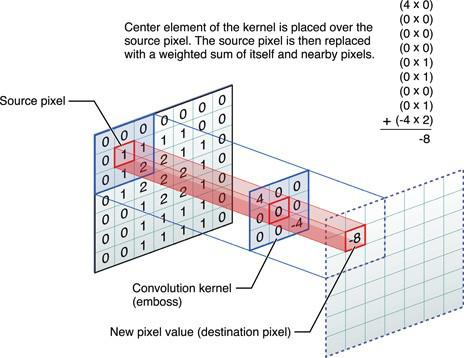
\includegraphics[width=8cm]{img/convolutionAssignment.jpg}
    \caption*{Figure 1: Example of 2D convolution for emboss, reproduced from [8].}
\end{figure}

The task is to design and implement a processor that is optimized to perform convolution operation on data with two dimensional structure (e.g. images).

\subsubsection{Additional requirements}
Your processor will be implemented on an FPGA, and you are free to choose how to realize  your computer architecture.
Studying the architecture of general multi core processors [6], and parallel machines options [4, 5, 6, 7] can be a good starting point.

The task should also include a suitable application that can process/produce graphical data. 
The output is to be displayed in order to demonstrate the processor. 

The unit must utilize a Silicon Labs EFM32 series microcontroller (to act as an I/O processor) and a Xilinx FPGA (to implement your architecture on).
The budget is 10.000 NOK per group, which must cover components and PCB production. 
The unit design must adhere to the limits set by the course staff at any given time.
Deadlines are given in a separate time schedule.

And a final tip; Keep it simple, as simple as possible, but not simpler.

\subsubsection{References}
\begin{enumerate}
    \item M Flynn; Some Computer Organizations and Their Effectiveness; IEEE Transactions on Computers. Volume:C 21 ,  Issue: 9. 1972
    \item Qadeer, et al.; Convolution Engine: Balancing Efficiency \& Flexibility in Specialized 
Computing. Proceding of ISCA 2013, ACM 2013. 
http://csl.stanford.edu/~christos/publications/2013.convolution.isca.pdf  (Slides from 
presentation:\\ 
http://csl.stanford.edu/~christos/publications/2013.convolution.isca.slides.pdf)
    \item Open VG: https://www.khronos.org/openvg/ 
    \item Bell et al.; TILE64 Processor: A 64 Core SoC with Mesh Interconnect; ISSCC; 20M 
Flynn; Some Computer Organizations and Their Effectiveness; IEEE Transactions on 
Computers. Volume:C 21, Issue: 9. 1972
    \item Kongetira et al.; Niagara: A 32 way Multithreaded SPARC Processor; IEEE MICRO; 
2005
    \item Wikipedia; Goodyear MPP; http://en.wikipedia.org/wiki/Goodyear\_MPP
    \item Borkar and Chien; The Future of Microprocessors; Communications of the ACM; 
2011.
    \item http://www.westworld.be/convolution kernels/
    \item http://www.ke5fx.com/crt/8753aft.jpg
\end{enumerate}
\end{quotation}
